\chapter{Materials and Methods} \label{cap:materials}


% 4. Challenges and Trends
% Sensor sensitivity, calibration, and reliability (e.g., SAW, LiDAR challenges).
% Power management and energy harvesting (e.g., Beat Sensors).
% Communication constraints in remote areas.
% Cybersecurity in embedded WSN devices.
% LMM and AI uses examples AI/ML for anomaly detection, forecasting.
% Edge computing trends.
% Scalability.
% Battery life and energy harvesting.
% Integration with cloud and AI pipelines

% In RF, SAW is fully consolidated. In environmental and chemical sensing, it is still a highly active research area with limited commercialization. attempt to resume: ”SAW shows high potential for environmental monitoring, especially for miniaturized, high-sensitivity applications, but adoption is still mostly at the experimental or niche industrial level.” 


To achieve the proposed objectives in this project, the work is divided into a few phases. In the first phase tests will be conducted in a controlled environment to evaluate the different sensors performance, without interferences form the network connection elements or variations in environmental conditions. In this phase the sensors will be integrated into a microcontroller-based sensor node and classified to define the best sensor for the application in monitoring a large river, such as the Itajaí-Açu river, and the most cost efficient solution for a smaller channel/river. In this phase the sensors will be tested, with the goal of evaluating their performance in terms of accuracy, precision, range, resolution, and susceptibility to common interferences such as temperature shifts, target surface variations, and water conditions. 

On a second phase, the sensor nodes will be connected to a \gls{LoRa} / \gls{LoRaWAN} network, and the data will be transmitted to a backend database for storage and visualization. The network will be designed to operate in a star topology, with one central gateway and multiple sensor nodes. The sensor nodes will be programmed to periodically make multiple readings on the distance data, process it and send  to the gateway using \gls{LoRa} modulation.

Finally, the system will be deployed in a real environment, such as a river or water body, to evaluate its performance in terms of data accuracy, transmission success rate, energy efficiency, and resilience against ambient environmental conditions. The collected data will be analyzed to provide insights into the performance of the sensors and the overall system.

\section{System Architecture}
The proposed monitoring system is built around a modular \gls{WSN} designed for remote water level monitoring. Each node in the network is equipped with non-contact distance sensors, \gls{LiDAR} and/or ultrasonic, and a \gls{LoRa}/\gls{LoRaWAN} communication module. The architecture comprises the following subsystems:

\begin{itemize}
\item \textbf{Data Acquisition}: Utilizes \gls{LiDAR} and/or ultrasonic sensors for distance measurement.
\item \textbf{Processing Unit}: A low-power microcontroller (e.g., ESP32, ESP8266) reads sensor data and manages system logic.
\item \textbf{Communication Interface}: Sends processed data via \gls{LoRa}/\gls{LoRaWAN} to a centralized gateway.
\item \textbf{Power Management}: Employs rechargeable batteries and optional solar panels.
\end{itemize}

\section{First Phase: Sensor Testing and Calibration} 

Sensors are mounted on adjustable rigs to test performance against fixed surfaces at various distances and materials. Environmental conditions like ambient temperature and lighting are controlled.

\subsection{Microcontroller Unit}
A low-power microcontroller such as the ESP8266 is selected for this project due to its sufficient performance, integrated Wi-Fi, and support for external LoRa modules. The MCU interfaces with sensors using UART,I2C and digital I/O.

This microcontroller will be used throughout the project, from the first phase of testing the sensors to the final deployment in the field. It will be responsible for reading sensor data, processing it, and transmitting it via LoRa. The microcontroller will also be responsible for managing power consumption, entering a low-power sleep mode when not actively collecting or transmitting data.

\subsection{Sensors}
Four distance sensors were used to capture water level data for performance comparison:
\begin{itemize}
\item \textbf{TF-Luna (\gls{LiDAR})}: Compact, accurate, and low-cost, with up to 8 m range.
\item \textbf{TF-Nova (\gls{LiDAR})}: Offers improved range (up to 12 m) and stability over TF-Luna.
\item \textbf{JSN-SR04T (Ultrasonic)}: Waterproof, outdoor-suitable sensor with 6 m range.
\item \textbf{HC-SR04 (Ultrasonic)}: Basic sensor for initial prototyping, up to 4 m range.
\end{itemize}

The four sensors will be tested in the same conditions, connected to a ESP8266 microcontroller, which will read the data and send it to a connected computer for analysis. After the tests are completed the data will be analyzed to determine the best sensor for the application, considering factors such as cost, performance, and environmental conditions.

The list of tests to be performed was defined based on the sensors specifications, the project requirements and based on some findings of previous works, \cite{paul_2020_a} found that the temperature can affect the readings of the \gls{LiDAR} sensors, and \cite{tamari_2016_flash} mentions that future works should look  to check if the number of suspended small particles in the water could impact the readings of \gls{LiDAR} sensors. The tests will be as follows:

\begin{itemize}
    \item \textbf{Distance Range Test}: Sensors are tested at various distances to detect soft and hard reading limits.
     \item \textbf{Precision Test}: Multiple readings are taken at fixed distances to evaluate precision.
     \item \textbf{Accuracy Test}: Comparing sensor readings with reference measurements to determine accuracy.
     \item \textbf{Light Interference Test}: Sensors are tested under different lighting conditions to assess sensitivity to ambient light.
     \item \textbf{Surface Material Test}: Sensors are tested on different surfaces (clean water, water mixed with earth, solid materials).
     \item \textbf{Temperature Variation Test}: Sensors are tested at different temperatures.
     \item  \textbf{Environmental Interference Test}: Sensors are tested in simulated and controlled envirmental conditions with wind, rain, and other environmental factors.
\end{itemize}

\section{Second Phase: System Integration and Communication}

After evaluating the sensors, the selected ones are integrated into a sensor node. Besides the sensor, the node includes the LoRa transceiver, a microcontroller, and a power management system.  The node is programmed to read sensor data, process it, and transmit it via LoRa. The node is designed to operate in low-power mode, waking up at set intervals to collect and send data.

\subsection{Communication Module}
A LoRa transceiver operating at 915 MHz enables long-range data transmission with minimal energy consumption. Each node sends data to a gateway(LoRa Receiver) which forwards it to a backend database for storage and visualization. Figure \ref{fig:node_integration_diagram} illustrates the integration of the LoRa nodes and the receiver.

\begin{figure}[h]
    \centering
    \caption{LoRa Nodes and Receiver integration diagram.}
    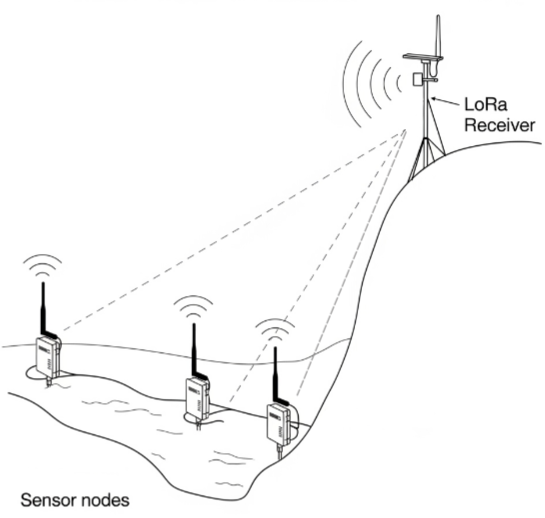
\includegraphics[width=0.65\textwidth]{figuras/lora_nodes_and_receiver.PNG}
    \fonte{The author.}
    \label{fig:node_integration_diagram}
\end{figure}

\section{Third Phase: Field Deployment and Evaluation}

\subsection{Field Deployment}
The complete system is deployed near a river or water body. Each node is securely housed and positioned above the water surface.
\begin{itemize}
\item Evaluation criteria: data accuracy, transmission success rate, energy efficiency, and resilience.
\item Nodes report data every 15 minutes; timestamps allow trend tracking.
\end{itemize}

\subsection{Node Software Architecture}
The software architecture is designed to ensure efficient data acquisition, processing, and transmission. The main loop reads sensor data, processes it, and transmits packets via LoRa only in set intervals to conserve energy, entering a deep sleep state otherwise. The flow of the node while it is active is descrbed in Figure \ref{fig:sensor_node_software_diagram}.	

\begin{figure}[h]
	\centering
	\caption{Sensor node diagram.}
	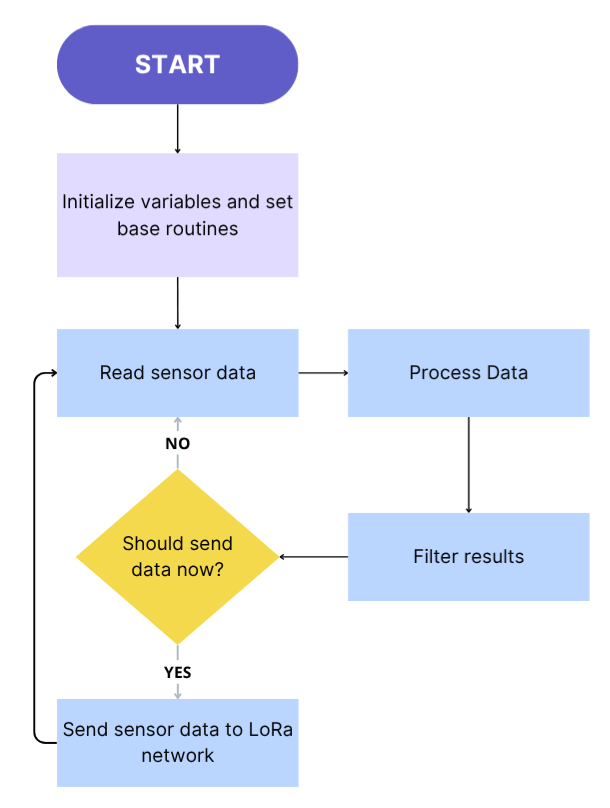
\includegraphics[width=0.65\textwidth]{figuras/sensor_node_software_diagram.PNG}
	\fonte{The author.}
	\label{fig:sensor_node_software_diagram}
\end{figure}

\subsection{Data Communication and Network Topology}
Each node periodically collects distance data and sends it to the gateway using LoRa modulation. The gateway relays this data to a server through Wi-Fi or cellular connection. The network is structured in a star topology with one central gateway and multiple sensor nodes.

\section{Data Processing and Storage}
Received sensor data is stored in a cloud database for further analysis. Time-series data is cleaned and visualized using statistical and signal processing tools. Metrics such as mean, standard deviation, and RMSE are computed.

\section{Expected Outcomes}
This integrated system aims to evaluate the accuracy, stability, and cost-effectiveness of multiple distance sensors in real-world hydrological monitoring. The LoRa-based architecture enables remote deployment and real-time water level reporting, supporting early warning and sustainability goals. 

\begin{figure}[h]
	\begin{lstlisting}[caption={Exemplo de um schema no Prisma.}, label={code:prisma}]
	generator client {
		provider = "prisma-client-js"
	}
	
	datasource db {
		provider = "postgresql"
		url      = env("DATABASE_URL")
	}
	
	model User {
		id        String        @id @unique @default(uuid())
		email     String        
		password  String
		cpf_cnpj  String        @unique
		name      String
		role      RoleEnumType? @default(user)
		createdAt DateTime      @default(now())
		updatedAt DateTime      @updatedAt
	}
	
	enum RoleEnumType {
		user
		admin
	}
		
	\end{lstlisting}
	
	\fonte{The author.}
	\end{figure}


\begin{table}
	\ABNTEXfontereduzida
	\caption{\label{tab:Tab_2}Table comparing sensors.}
 \begin{center}
	\begin{tabular}{@{}p{2.0cm}p{2cm}p{2.5cm}p{2cm}p{2.0cm}@{}}
		\toprule
		\textbf{Sensor} & \textbf{Type} & \textbf{Range} & \textbf{Precision} & \textbf{Accuracy} \\ \midrule
		JNS SR04T & Ultrasonic & 20 cm a 4 m & ±1 cm  & ±1 cm \\
		HC-SR04 & Ultrasonic & 2 cm a 4 m & ±3 mm  & ±3 mm \\
		TF-Luna & \gls{LiDAR} & 0,2 m a 8 m & ±1 cm   & ±1 cm \\
		TF-Nova & \gls{LiDAR} & 0,1 m a 12 m & ±1 cm  & ±1 cm \\
  \bottomrule
	\end{tabular} 
 \end{center}
	\fonte{The author.}
	\label{tab:comparativo}
\end{table}
